% ===============================
% Data collection
% ===============================
\newpage
\section{Data}
\label{sec:datacollection}

When gathering data for behavioural analysis of different species, typically the observer tracks the position of one or several individuals over the time. Additionally pheno- and genotypical data of the individuals is collected.

Usually the spatial postion data is collected by one ore a few people. In this project the data is collected by an antenna system (see section \ref{subsec:collectspatialpos} on page \pageref{subsec:collectspatialpos}). This approach has the advantage, that the data is recorded 24 hours a day, without presence of people needed.

To collect phenotypical data, so called \textit{population checks} (see \ref{subsec:dataattr} on page \pageref{subsec:dataattr} for details) are conducted every 6 to 8 weeks. During these checks, the mice get caught for measuring, weighing (see section \ref{subsec:dataattr} on page \pageref{subsec:dataattr} for details) and - if not already present and the mouse has a weight of at least 18 grams - an \ac{RFID} (RFID) transponder is injected under the skin of the mouse (see figures \ref{fig:transponder} and \ref{fig:inject_rfid}). About 240 transponders are injected every Year.

\begin{figure}[htpb]
\begin{center}
		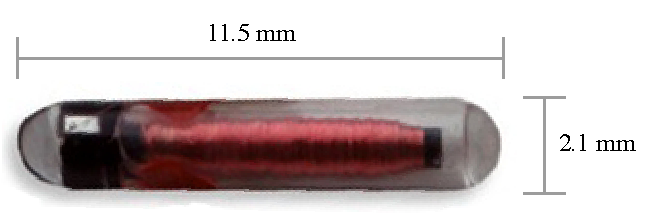
\includegraphics[width=0.5\textwidth]{assets/pdf/transponder.pdf}
  		\caption[Trovan ID-100A Microtransponder]{Pictured an ID-100A Microtransponder from $Trovan^{\copyright}$. The transponder weighs 0.1 g and the coat is made of biocompatible glass.\newline \small Picture courtesy of Trovan.}
  		\label{fig:transponder}
\end{center}
\end{figure}
\begin{figure}[htpb]
\begin{center}
		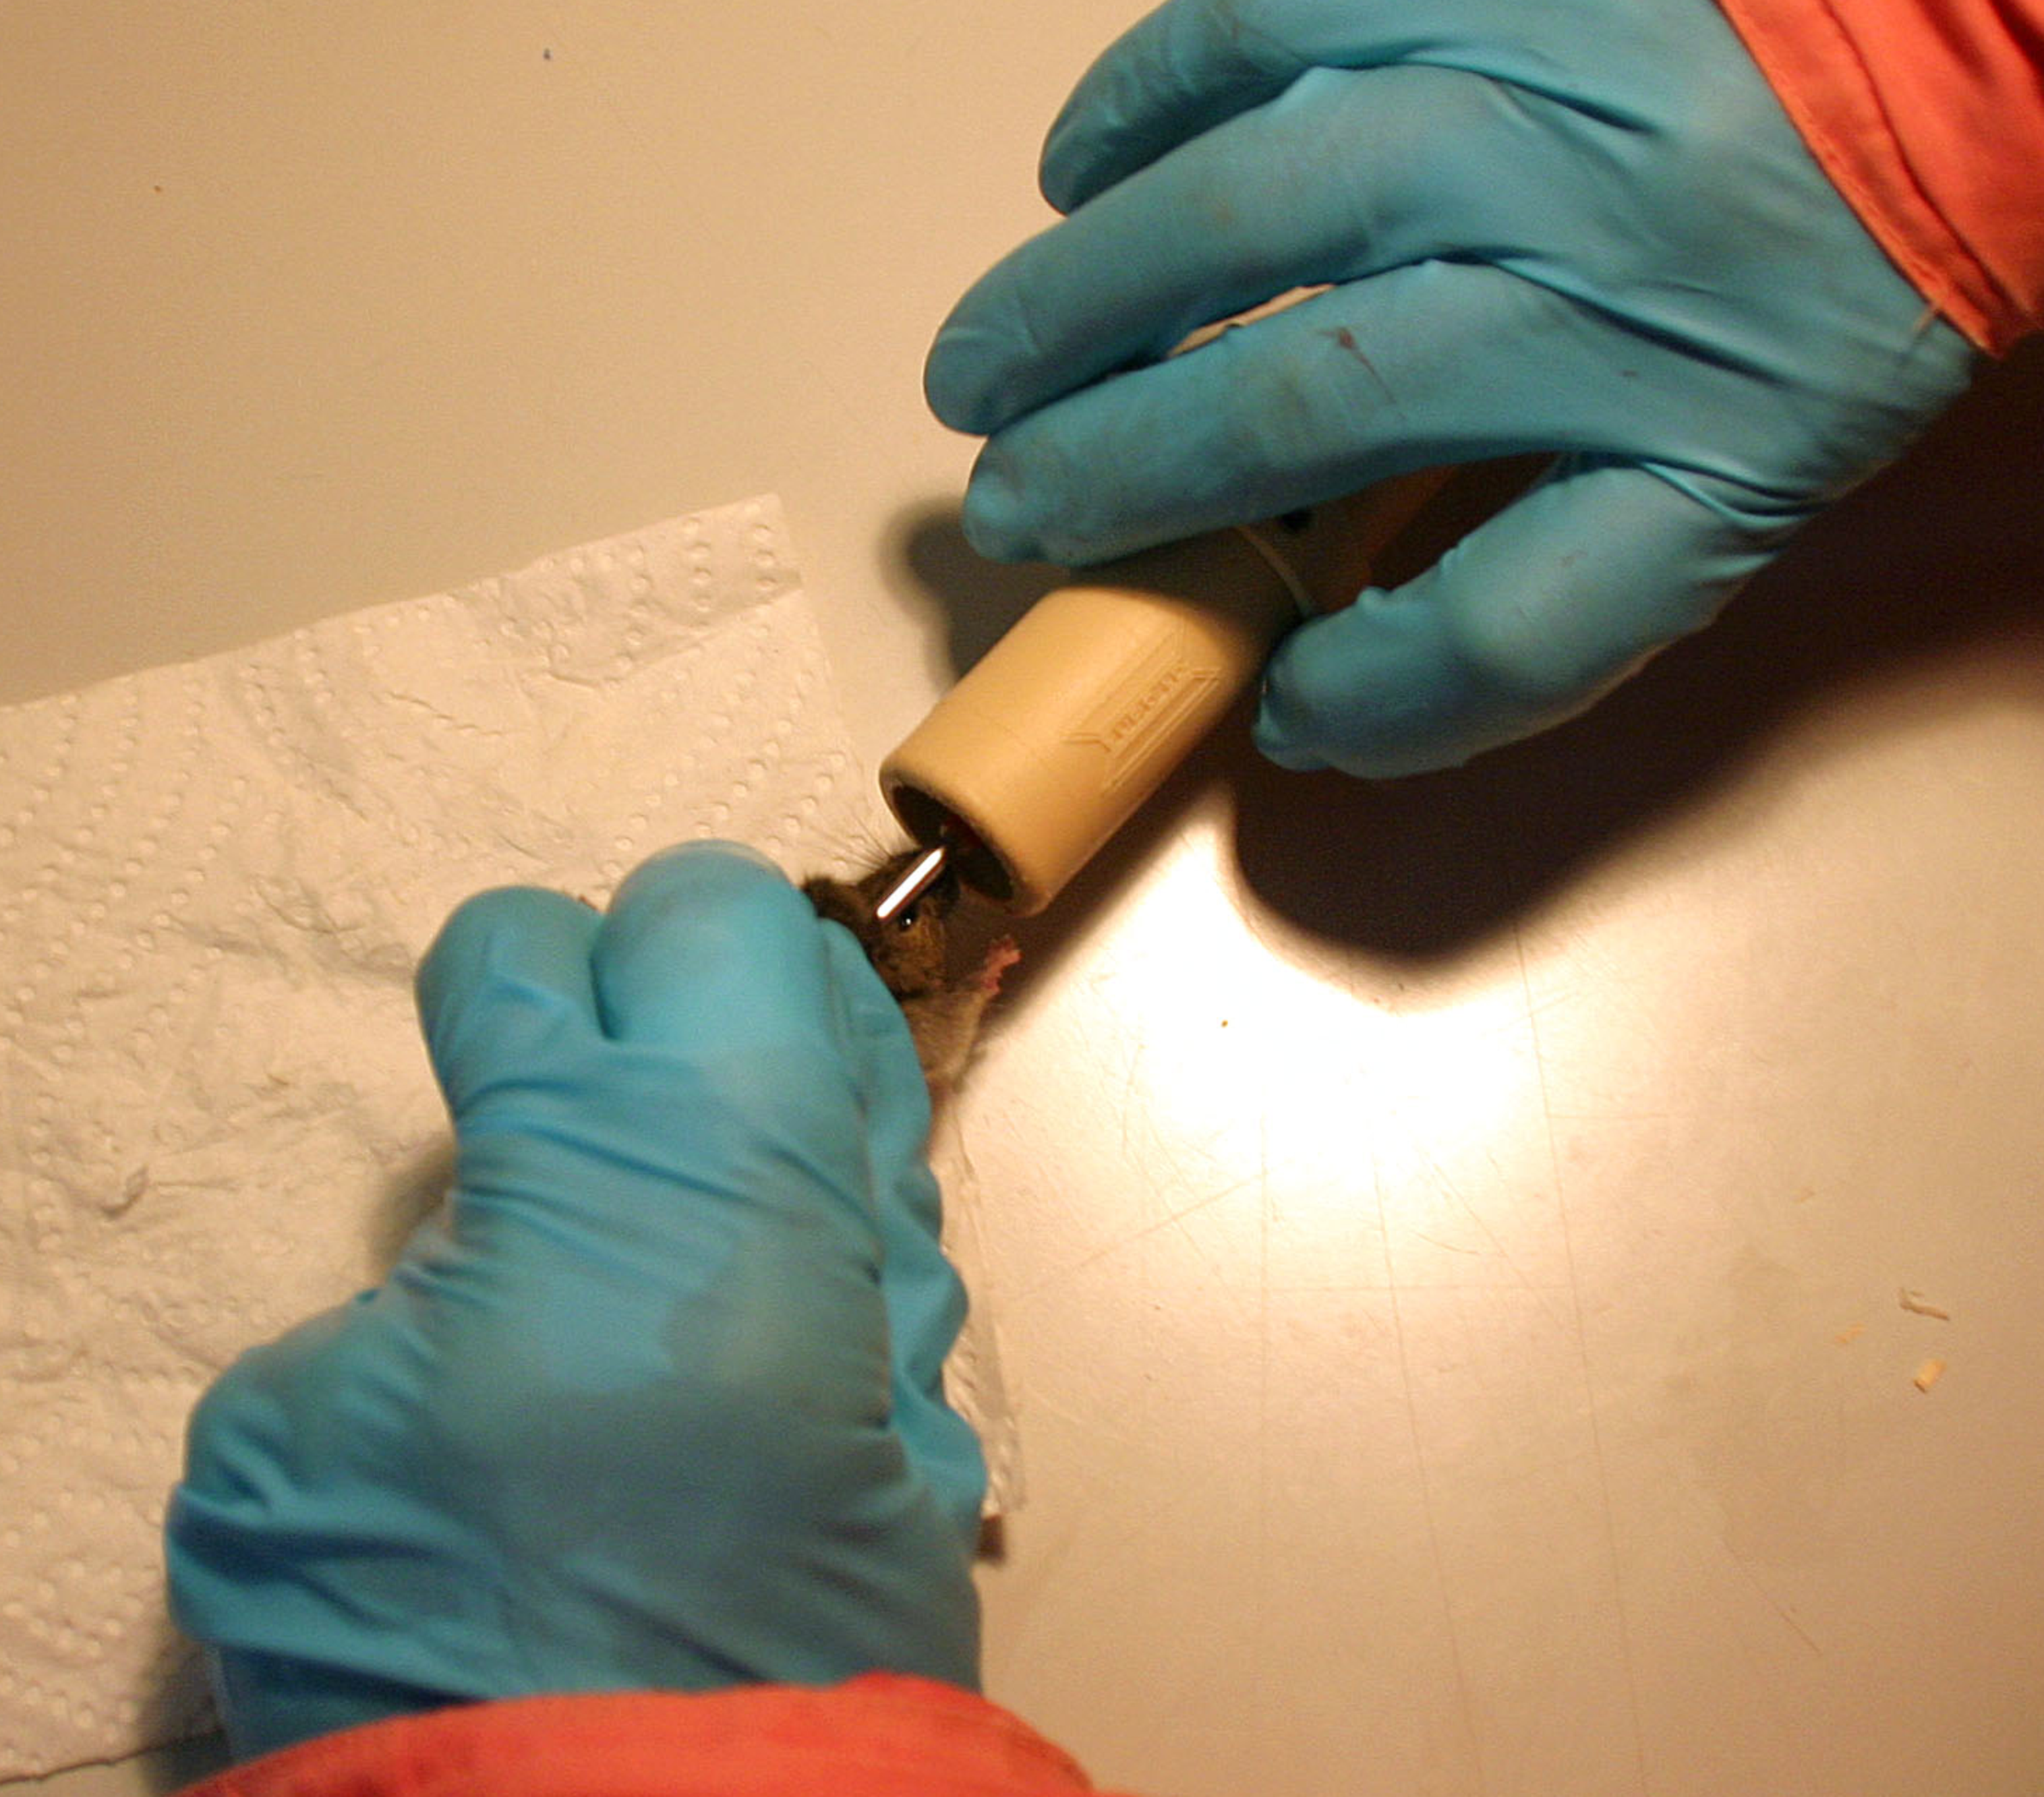
\includegraphics[width=0.5\textwidth]{assets/pdf/transponder_inject.pdf}
  		\caption[Injecting an RFID transponder]{Subcutaneous injection of an RFID transponder.}
  		\label{fig:inject_rfid}
\end{center}
\end{figure}

The genetical information is needed to get information about the relatedness between the mice within the population. Genotypical information is not included in the data used for this work.

%----------------------------------------------
%Position / Time data
% ----------------------------------------------
\subsection{Collecting spatial position data}
\label{subsec:collectspatialpos}

To collect the spatial position data, a project specific system has been by built by \textit{New Behaviour}, a company specialized in creating systems to study animal behaviour. 

The basic idea is to use \acf{RFID} transponders, to identify the mice at specific locations in the shed. These \ac{RFID} transponders are about the size of a rice corn and are injected under the skin of the mice (see figure \ref{fig:inject_rfid} on page \pageref{fig:inject_rfid}). 

Furthermore, the system includes 40 artificial nestboxes, made of \ac{PVC}, which have a diameter and a height of 15 centimeters. The entry tube is about 20 to 25 centimeters long, made of \textit{Plexiglass}, and is bent by an angle of 45 degrees to slow down the mice when they go trough the pipe (see fig. \ref{fig:artNestbox} on page \pageref{fig:artNestbox}). This is improving the accuracy of the two antennas which are wrapped around the tube and read the RFID transponders. The antennas have a coverage area with a radius of about 10 to 12 centimeters.
 
\begin{figure}[htbp]	
\centering	
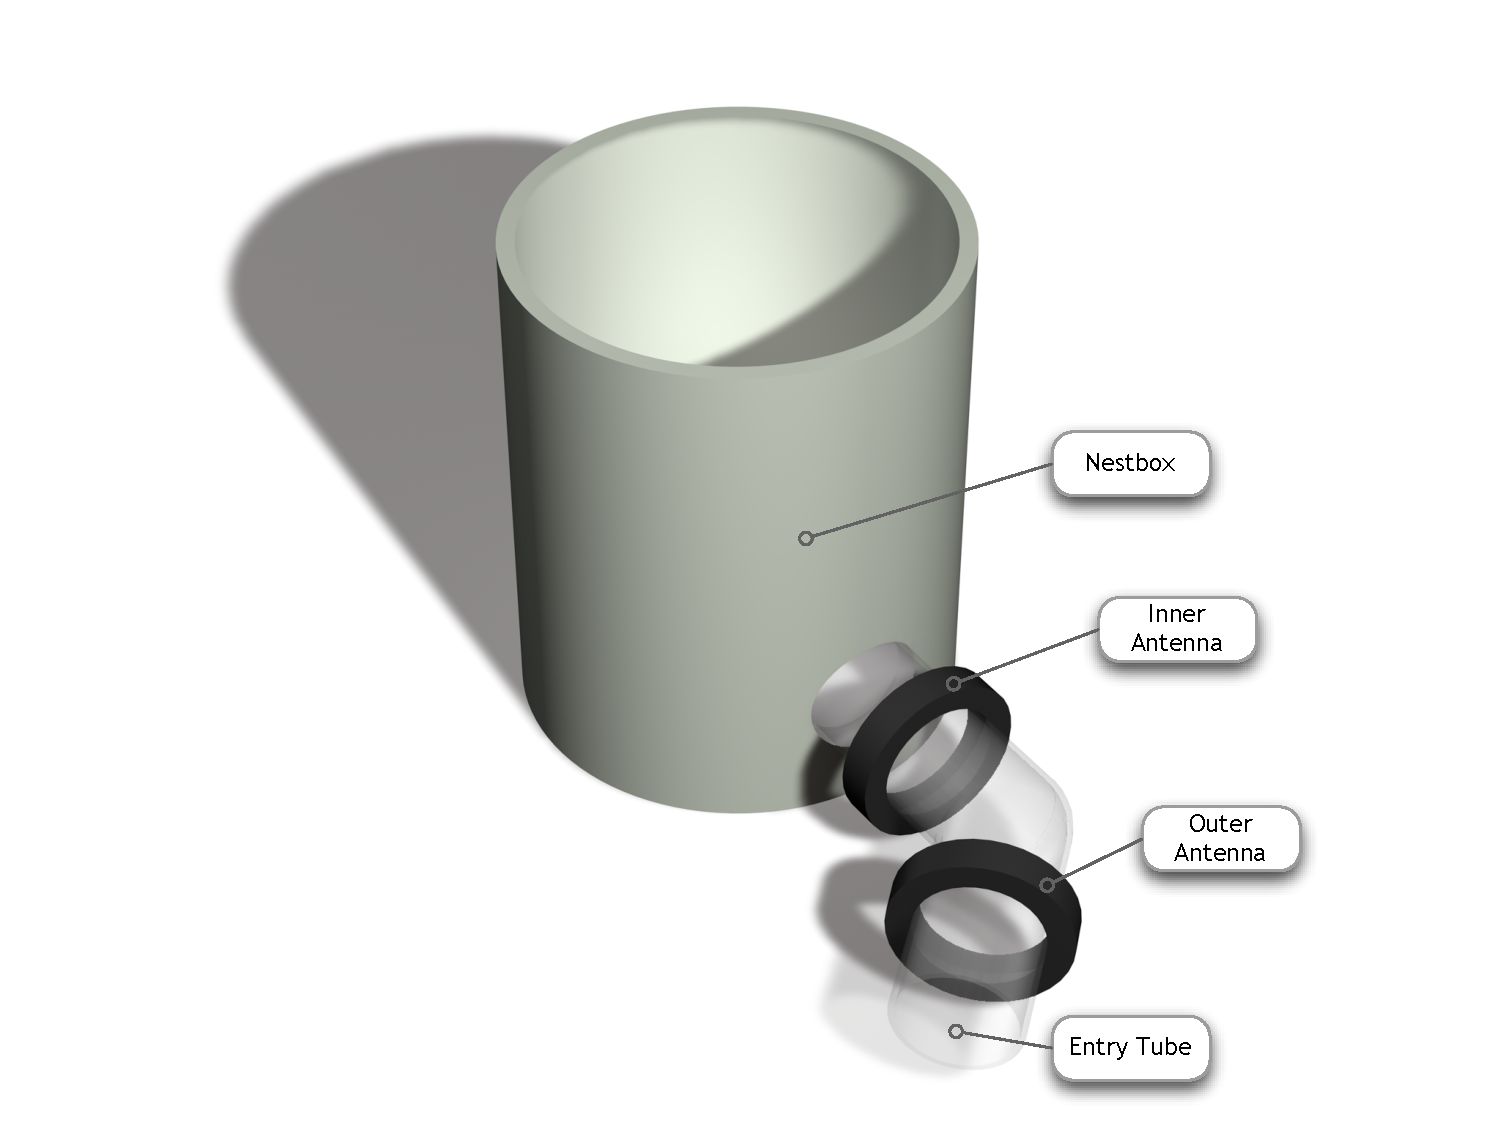
\includegraphics[width=0.75\textwidth]{assets/pdf/box_schema.pdf}	
\caption[Model of an artificial nestbox]{3d-Model of an artificial nestbox with the two antennas wrapped around the entry tube.}
\label{fig:artNestbox}
\end{figure}

The \ac{RFID} transponders used are passiv, meaning that they do not include a battery. The antenna acts as a scanner, presenting an inductive field which excites the \ac{RFID} transponder when entering the coverage area of the antenna. This energy is used by the transponder to send its identification to the antenna. 

So, whenever a mouse carrying a transponder passes by an antenna, it's identification is recorded and sent to a central computer along with the antenna adress. The computer then writes the received data to a text file. The structure of these data files is explained in detail in the next section.

\subsubsection{Data File Format}
\label{subsubsec:datafileformat}
The data files are simple text files, where each line denotes an \textit{event} registered by an antenna in the system. Every day the data file is closed, saved, and a new data file is created automatically by the system.

Basically there are to types of events. The system output for first type is shown in figure \ref{fig:dataset} on page \pageref{fig:dataset}. It shows the line of text written to the data file when the \ac{RFID} transponder has been identified by an antenna. The id of the transponder is a unique, ten character wide, alphanumeric value.

\begin{figure}[htbp]	
\centering	
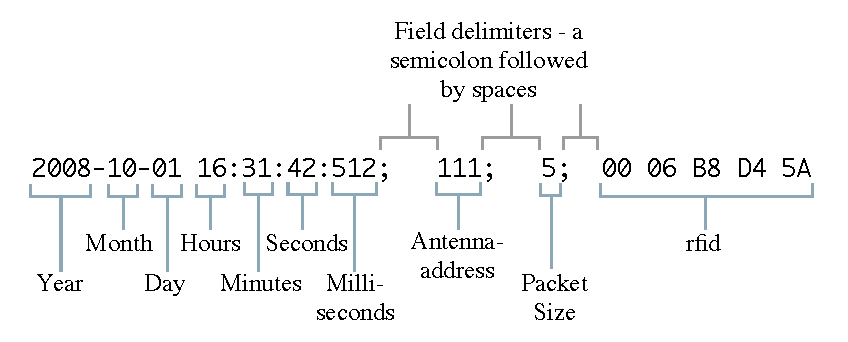
\includegraphics[width=0.8\textwidth]{assets/pdf/dataset.pdf}	
\caption[Dataset with RFID transponder identification]{Typical dataset in a data file with and \ac{RFID} transponder identification}
\label{fig:dataset}
\end{figure}

If a transponder enters or leaves the coverage area of an antenna, the second event type occurs. The ouput is shown in figure \ref{fig:dataset_no_data} on page \pageref{fig:dataset_no_data}.

\begin{figure}[htbp]	
\centering	
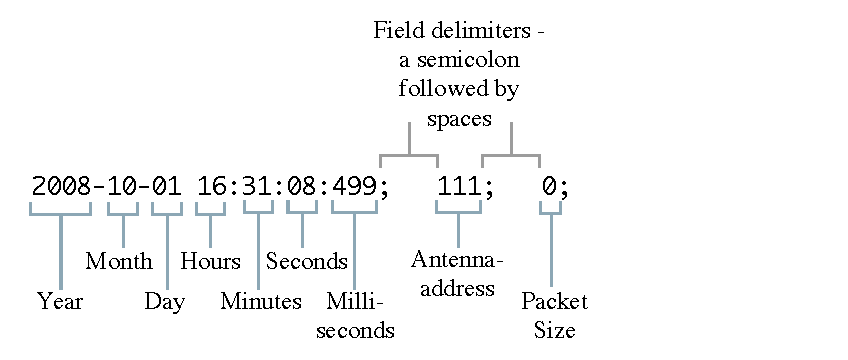
\includegraphics[width=0.8\textwidth]{assets/pdf/dataset_no_data.pdf}	
\caption[Dataset without RFID transponder identification]{Typical dataset in a data file without an \ac{RFID} transponder identification}
\label{fig:dataset_no_data}
\end{figure}

The following lines show the data written to the data file by the system, when a mouse passes the two antennas attached to a box. The events taking place when each of these lines is written to the data file is explained in the following list. The list numbers match the line numbers of the data file fragment. 

\numcodestyle
\begin{lstlisting}[frame=none]
2008-10-01 16:31:08:499;   111;   0; 
2008-10-01 16:31:09:095;   113;   0; 
2008-10-01 16:31:42:512;   111;   5;  00 06 B8 D4 5A
2008-10-01 16:31:42:807;   113;   5;  00 06 B8 D4 5A
2008-10-01 16:31:43:619;   111;   0; 
2008-10-01 16:31:44:014;   113;   0;
\end{lstlisting}

\begin{condensed_enum}
  \item The transponder \textbf{enters coverage area} of the antenna with address \lstinline|111|.
  \item The transponder \textbf{enters coverage area} of the antenna with address \lstinline|113|.
  \item The transponder is \textbf{identified} as \lstinline|00 06 B8 D4 5A| at antenna with address \lstinline|111|.
  \item The transponder is \textbf{identified} as \lstinline|00 06 B8 D4 5A| at antenna with address \lstinline|113|.
  \item The transponder \textbf{leaves coverage area} of the antenna with address \lstinline|111|.
  \item The transponder \textbf{leaves coverage area} of the antenna with address \lstinline|113|. 
\end{condensed_enum}
 
Depending on the event type, the value of the packet size is either a \lstinline|0| for events without a transponder identification value, or a \lstinline|5| if the transponder has been identified. For the data processing (see section \ref{sec:dataproc} on page \pageref{sec:dataproc}) only the datasets with a transponder identification are taken into account.

\subsubsection{Antenna adressing}
\label{subsubsec:addressing}

There are always two antennas attached to an entry tube of a box (see figure \ref{fig:artNestbox} on page \pageref{fig:artNestbox}). The antenna address is three digits long, composed by the box number it is attached to (first two digits), and the position at the entry tube of the box. Outer antennas have a \lstinline|1| as the last digit of the address, innner antennas a \lstinline|3| (e.g the antennas attached to box 11 are addressed 111 for the outer, 113 for the inner antenna, respectively). Needless to say, that box numbers have to be unique.

Unfortunately there are a few exceptions to that schema, as for a few antennas, the correct addressing failed due to technical problems (cp. \ref{subsubsec:problems} at page \pageref{subsubsec:problems}).

\subsubsection{General system design and functionality}
\label{subsubsec:generalsystem}

\begin{itemize}
  \item Can-Bus
  \item cable loop
  \item rfid identification how
  \item What happens in the boxes (boards) next to the antennas
  \item How is can bus working/implemented
  \item Where are the different cable loops (which antennas connected to a loop)
  \item General system layout (cabeling, protocols)
  \item Programmed software
  \item etc. 
\end{itemize}

\subsubsection{Problems}
\label{subsubsec:problems}

Unfortunately the problems with the system are diverse. Antenna drop outs, broken laptop or cable connections chewed by the mice, to name just a few. Some of these problems could be solved, other still remain.

However, one of biggest problem is, that the readings at the antennas are not as reliable as planned. This is clearly visible in the following numbers:

From the 5 of April 2007 to the 27 of March 2009, xxx datasets (table \lstinline|data|) have been recorded. Assuming that the system works perfect, we would get xxx \textit{direction results}. Compared to the real number of \textit{direction results}, which is xxx, we have a yield of xx\%.

In the next step, two \textit{direction results} should create a \textit{stay result}. The script which searches for the \textit{stay results} could find xxx results in the xxx \textit{direction results}, which is xx\%. Most likely this low numbers are an effect of missed antenna readings. Normally, an antenna reads out the transponder information 10 times, to ensure maximum 

Another problem are the transponders which have never been injected in a mouse, but are recorded by the system. 

\numcodestyle
\begin{lstlisting}[frame=none]
2007-11-25 10:09:12:906;   381;   5;  00 06 B8 E2 70
2007-11-25 10:09:16:529;   381;   5;  00 05 B8 D2 70
2007-11-25 10:09:16:932;   381;   5;  00 06 B8 E2 70
2007-11-25 10:09:19:950;   381;   0; 
2007-11-25 10:09:20:253;   381;   5;  00 06 B8 E2 70
\end{lstlisting}   

This clipping of a data file shows an \ac{RFID} transponder which appears as \lstinline|00 05 B8 D2 70| on line two but as \lstinline|0 06 B8 E2 70| on the other data lines. The \lstinline|rfid| table contains xxx different \ac{RFID}'s whereof xxx could not be identified as an injected transponder.   

Furthermore, for some antennas the address could not be set properly. In one case two antennas even sent the same adress, so that no distinction of the data could be made. The workaround for this problem is, two find an unused address which we are able to set and map it to the desired address during the data import.   

% ----------------------------------------------
%Data attributes
% ----------------------------------------------
\subsection{Collecting Data Attributes}
\label{subsec:dataattr}

During the \textit{population checks}, the whole shed, including all artificial nestboxes, plastic pipes and other structuring elements, is checked to screen the mice population. During these so called population and nest checks the data is collected using the following procedure.

\begin{enumerate} 
	\item Each box is opened and the following observations made:
	\begin{itemize}
      \item \textbf{Mice in the box:} If adult mice are in the box, they get identified by their transponder, measured and weighed. Furthermore it will be checked, if the sex of the mouse has already been determined.  
      \item \textbf{Bedding:} Determine if the nestbox shows marks of usage, like trampled bedding.
      \item \textbf{Pups:} Does the box contain pups, and if yes how many and whats their estimated age. 
      \item \textbf{Communal nest:} Check if two or more litters are reared in the box. 
    \end{itemize}
	\item All the possible shelters, like planks an pipes, are checked for mice presence as well.
\end{enumerate}

% ----------------------------------------------
%storing Data
% ----------------------------------------------
\subsection{Data storage}
\label{subsec:datastorage}

All the data is stored in a MySQL\footnote{\href{http://www.mysql.com/}{MySQL database}} database, which is  a \acf{RDBMS} (RDMS). The following figure (fig. \ref{fig:database_schema}) shows all the tables including the data types\footnote{An overview of the MySQL data types can be found on the following webpage: \url{http://dev.mysql.com/doc/refman/5.0/en/data-types.html}} of the columns and their relations to columns in other tables. 

A schema of the database including all the tables and the references between the table columns can be found in the Appendix on page \pageref{fig:database_schema_app}.


The tables can be divided into different groups by looking at the type of data they hold. The following sections explain these groups and the associated tables in short.

\subsubsection{Processed data}

This group comprehends tables with data based on the spatial position data collected by the system in the shed (see section \ref{subsec:collectspatialpos} on page \pageref{subsec:collectspatialpos} for details).

The tables belonging to that group are outlined in figure \ref{fig:processed_data_schema} on page \pageref{fig:processed_data_schema}.
 
\begin{figure}[htpb]
\begin{center}
  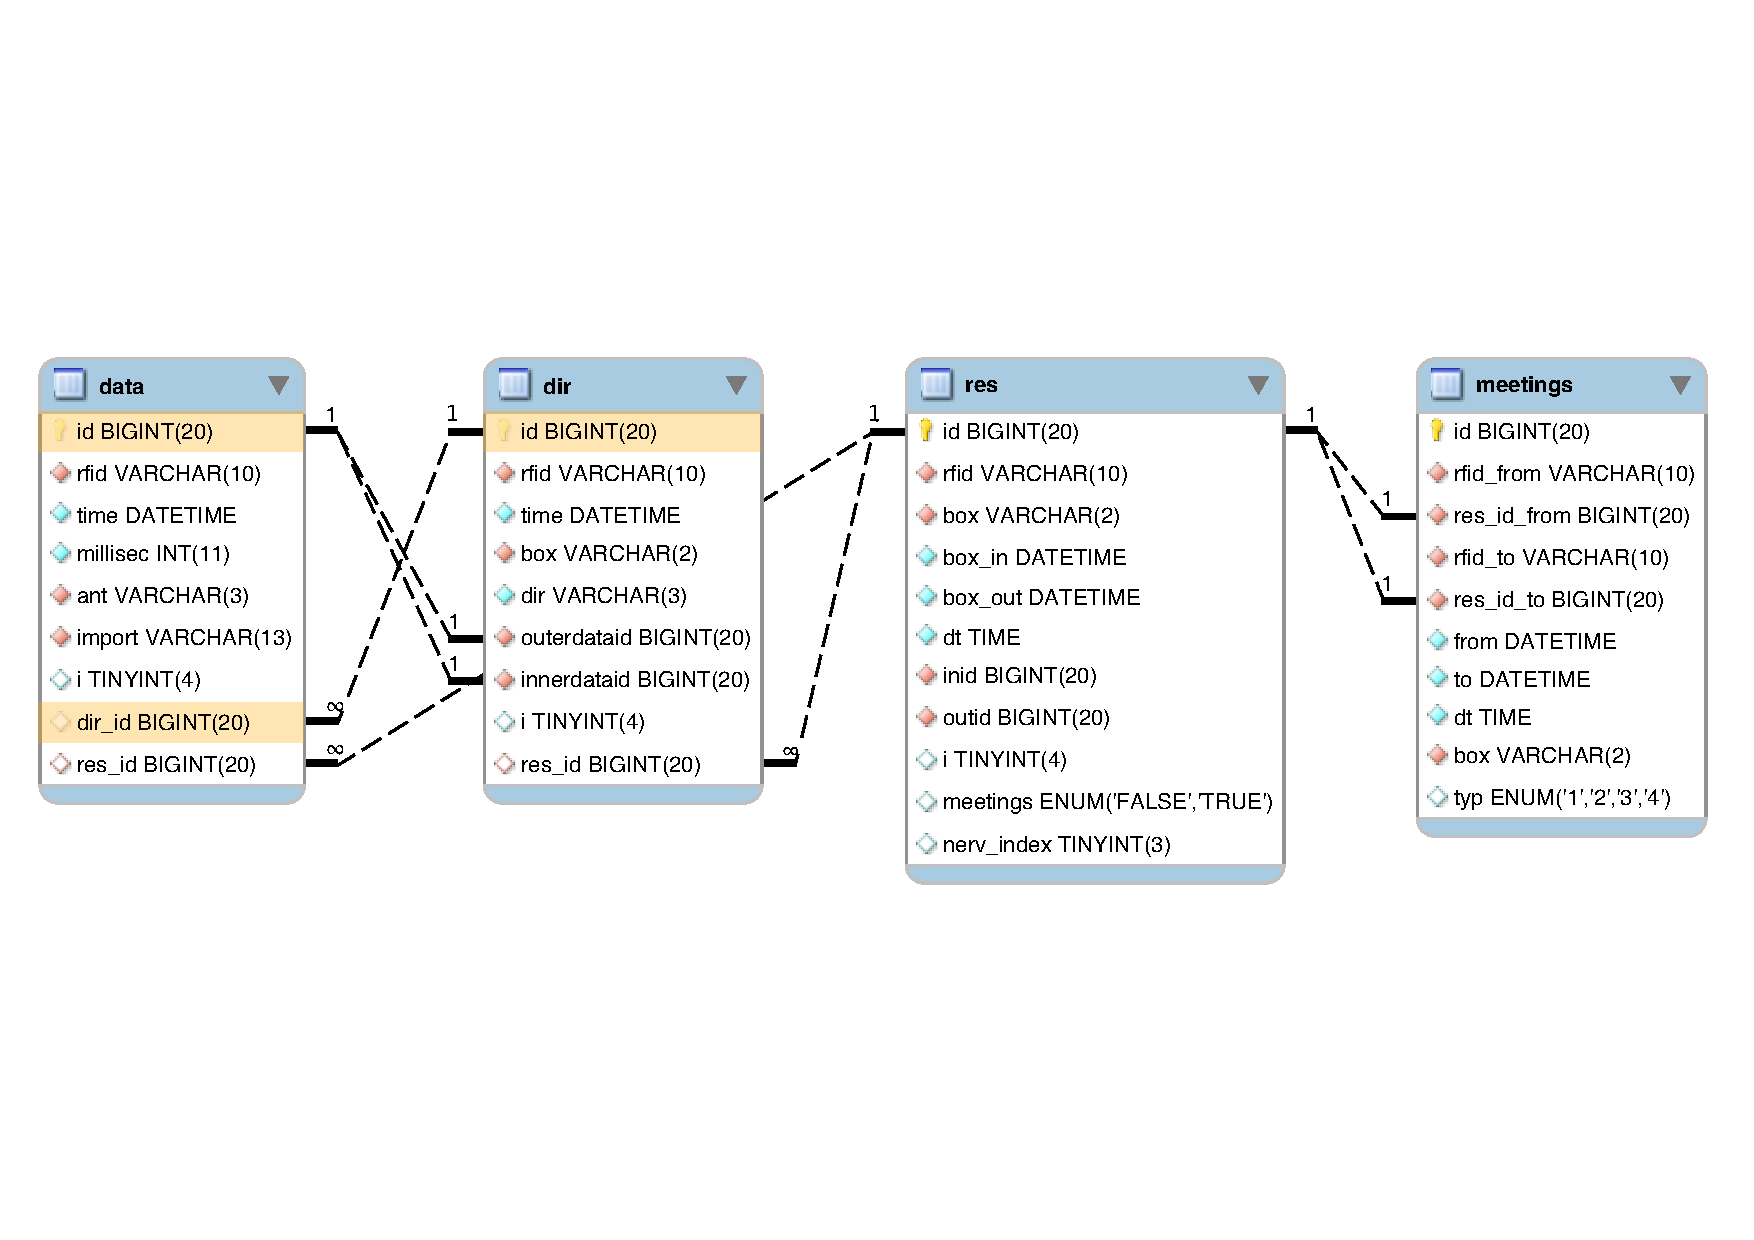
\includegraphics[width=\textwidth]{assets/pdf/processed_data_schema.pdf}
  \caption[Schema of database tables with processed data]{Schemata of the data tables with the processed spatial position data and the relations between them.}
  \label{fig:processed_data_schema}
\end{center}
\end{figure}

\paragraph{data table}
\label{para:data_table}

A \ac{perl} script imports the data files written by the system in the shed into the \lstinline|data| table. 

Shown next is a row of the \lstinline|data| table followed by short explanation of the columns.

\codescript
\begin{lstlisting}[frame=none]

(first part of table row)
+---------+------------+---------------------+----------+
| id      | rfid       | time                | millisec |
+---------+------------+---------------------+----------+
| 7321019 | 00069B4D4D | 2009-02-07 00:51:56 |      173 |
+---------+------------+---------------------+----------+

(second part of table row)
+-----+---------------+------+--------+--------+
| ant | import        | i    | dir_id | res_id |
+-----+---------------+------+--------+--------+
| 121 | 09-0206155809 |    4 |  40102 |  10001 |
+-----+---------------+------+--------+--------+

\end{lstlisting}

\begin{mydesc}
  \item \lstinline|id| is an auto increment integer and therefore a unique identifier of a dataset in this table.
  \item \lstinline|rfid| is a transponder value. This value is a reference to a value in the \lstinline|id| column of the \lstinline|rfid| table (see paragraph \ref{para:rfid_table} on page \pageref{para:rfid_table}).
  \item \lstinline|time| and \lstinline|millsec| columns harbor the time the dataset has been recorded. Unfortunately the \textit{MySQL} \lstinline|DATETIME| data type does not include the milliseconds. Hence, these values have to be stored in a seperate column.
  \item \lstinline|ant| denotes the antenna the data was recorded at. This value is a reference to a value in the \lstinline|id| column of the \lstinline|ant| table (see paragraph \ref{para:ant_table} on page \pageref{para:ant_table}).
  \item \lstinline|import| is a reference to a dataset in the \lstinline|logs| table, simply unveils from which data file this dataset is part of.
  \item \lstinline|i| is an indicator if the dataset could is used in a direction result (see \ref{para:dir_table} ) and stay result (see \ref{para:res_table}). Table \ref{tab:i_values} on page \pageref{tab:i_values} gives an overview of the \lstinline|i| values in the different tables.
  \item \lstinline|dir_id| is a reference to an \lstinline|id| in the \lstinline|dir| table, if that dataset could be used in a \textit{direction result}. Else, this value is \lstinline|NULL|.
  \item \lstinline|res_id| is a reference to an \lstinline|id| in the \lstinline|res| table, if that dataset could be used in \textit{stay result}. Else this value is \lstinline|NULL|.
\end{mydesc}

\paragraph{dir table}
\label{para:dir_table}
Another \ac{perl} script searches for matching pairs of datasets in the \lstinline|data| table which form a \textit{direction result}.

When a mouse carrying an \ac{RFID} transponder passes the two antennas attached to an artificial nestbox, within a certain time, it is possible to determine if the mouse went in or out of that box (see section \ref{subsec:dirres} on page \pageref{subsec:dirres} for details about the script). 

Shown next is a row of the \lstinline|dir| table followed by short explanation of the columns.

\codescript
\begin{lstlisting}[frame=none]

(first part of table row)
+-------+------------+---------------------+-----+-----+
| id    | rfid       | time                | box | dir |
+-------+------------+---------------------+-----+-----+
| 40102 | 00069B4D4D | 2009-02-07 00:51:56 | 12  | in  |
+-------+------------+---------------------+-----+-----+

(second part of table row)
+-------------+-------------+------+--------+
| outerdataid | innerdataid | i    | res_id |
+-------------+-------------+------+--------+
|     7321019 |     7321020 |    4 |  10001 | 
+-------------+-------------+------+--------+
\end{lstlisting}

\begin{mydesc}
  \item \lstinline|id| and \lstinline|rfid| have the identical function as in the \lstinline|data| table.
  \item \lstinline|time| denotes the moment the the \lstinline|rfid| entered or left the \lstinline|box|.
  \item \lstinline|box| is a reference to a value in the \lstinline|id| column of the \lstinline|box| table (see paragraph \ref{para:box_table} on page \pageref{para:box_table}).
  \item \lstinline|dir| is either \textit{in} or \textit{out} and depicts the direction.
  \item \lstinline|outerdataid| and \lstinline|innerdataid| values can be used to backtrack the datasets in the \lstinline|data| table making up the \textit{direction result}. This is explained in detail in section \ref{subsec:dirres} on page \pageref{subsec:dirres}.
  \item \lstinline|i| is an indicator if the direction result could is used in a \textit{} (see \ref{para:res_table}). Table \ref{tab:i_values} on page \pageref{tab:i_values} gives an overview of the \lstinline|i| values in the different tables.
  \item \lstinline|res_id| is a reference to an \lstinline|id| in the \lstinline|res| table, if that dataset could be used in \textit{stay result}. Else this value is \lstinline|NULL| (= empty).
\end{mydesc}

\paragraph{res table}
\label{para:res_table}

When two \textit{direction results}, one with a \lstinline|dir| value of \lstinline|in| and the other with a \lstinline|dir| value of \lstinline|out|, as well as matching \lstinline|rfid| and \lstinline|box| values are found, they form a so called \textit{stay result} (see section \ref{subsec:stayres} on page \pageref{subsec:stayres} for details).

Shown next is a row of the \lstinline|res| table followed by short explanation of the columns.

\codescript
\begin{lstlisting}[frame=none]

(first part of table row)
+-------+------------+-----+---------------------+---------------------+----------+
| id    | rfid       | box | box_in              | box_out             | dt       |
+-------+------------+-----+---------------------+---------------------+----------+
| 10001 | 00069B4D4D | 12  | 2009-02-07 00:51:56 | 2009-02-07 00:52:01 | 00:00:05 |
+-------+------------+-----+---------------------+---------------------+----------+

(second part of table row)
+----------+-------+---------+------+----------+------------+
| dt       | inid  | outid   | i    | meetings | nerv_index |
+----------+-------+---------+------+----------+------------+
| 00:00:05 | 40102 | 7321021 |    4 | TRUE     |          1 | 
+----------+-------+---------+------+----------+------------+

\end{lstlisting}

\begin{mydesc}
	\item \lstinline|id|, \lstinline|rfid| and \lstinline|box| were already explained for the previous tables, and have the same function in this table.
	\item \lstinline|box_in| and \lstinline|box_out| denote the beginning and the end time of the sojourn of the \lstinline|rfid| in a \lstinline|box|.
	 \item \lstinline|inid| and \lstinline|outid| can be used to backtrace the datasets in the \lstinline|dir| or \lstinline|data| table making up the \textit{stay result}. This is explained in detail in section \ref{subsec:stayres} on page \pageref{subsec:stayres}.
	 \item \lstinline|i| is either \lstinline|3| or \lstinline|4| and indicate the type of the result. This distinction is explained in detail in section \ref{subsec:stayres} on page \pageref{subsec:stayres}.
	 \item \lstinline|meetings| is set to \lstinline|true| when the result set has been analyzed for meetings.
	 \item \lstinline|nerv_index| gives an idea about how \textit{nervous} the mouse was when she stayed in the box. The \textit{nervousity} is explained in detail in section \ref{subsec:stayres} on page \pageref{subsec:stayres}. 
\end{mydesc}

\paragraph{meetings table}
\label{para:meetings_table}

In this work, an event is termed a \textit{meeting}, if \textit{stay results} of different mice in the same box show a temporal overlap. These meeting data are written to the \lstinline|meeting| table (see section \ref{subsec:meetingres} on page \pageref{subsec:meetingres} for details).

Shown next is a row of the \lstinline|meetings| table followed by short explanation of the columns.
\codescript
\begin{lstlisting}[frame=none]

(first part of table row)
++--------+------------+-------------+------------+-----------+
| id     | rfid_from  | res_id_from | rfid_to    | res_id_to |
+--------+------------+-------------+------------+-----------+
| 302635 | 0006CD478F |      596630 | 0006CC7962 |    596100 | 
+--------+------------+-------------+------------+-----------+

(second part of table row)
+---------------------+---------------------+----------+-----+------+
| from                | to                  | dt       | box | typ  |
+---------------------+---------------------+----------+-----+------+
| 2009-03-27 16:58:36 | 2009-03-27 17:01:00 | 00:02:24 | 13  | 1    |
+---------------------+---------------------+----------+-----+------+
\end{lstlisting}

\begin{mydesc}
	\item \lstinline|id| is the unique identifier of a dataset.
	\item \lstinline|rfid_from| and \lstinline|rfid_to| denote the two participating mice (\ac{RFID} transponders) of the \textit{meeting result}.
	\item \lstinline|res_id_from| points to the \lstinline|id| of the \textit{stay result} from the \lstinline|rfid_from|, and the \lstinline|res_id_to| to the one of the \lstinline|rfid_to|. This allows to look up the the \textit{stay results} making up this \lstinline|meeting result|.
	\item \lstinline|from|, \lstinline|to| and \lstinline|dt| declare the start, the end time and the duration of the meeting.
	\item \lstinline|box| contains the reference to an \lstinline|id| in the \lstinline|box| table (see \ref{para:box_table}).
	\item The different values of the \lstinline|typ| column are explained in detail in section \ref{subsec:meetingres} on page \pageref{subsec:meetingres}.
\end{mydesc}


\subsubsection{System members data}

This group encloses the tables wich contain data about the different \textit{members} of the data collection system in the shed.

The tables included in that group are outlined in figure \ref{fig:system_members} on page \pageref{fig:system_members}. 

\begin{figure}[htpb]
\begin{center}
  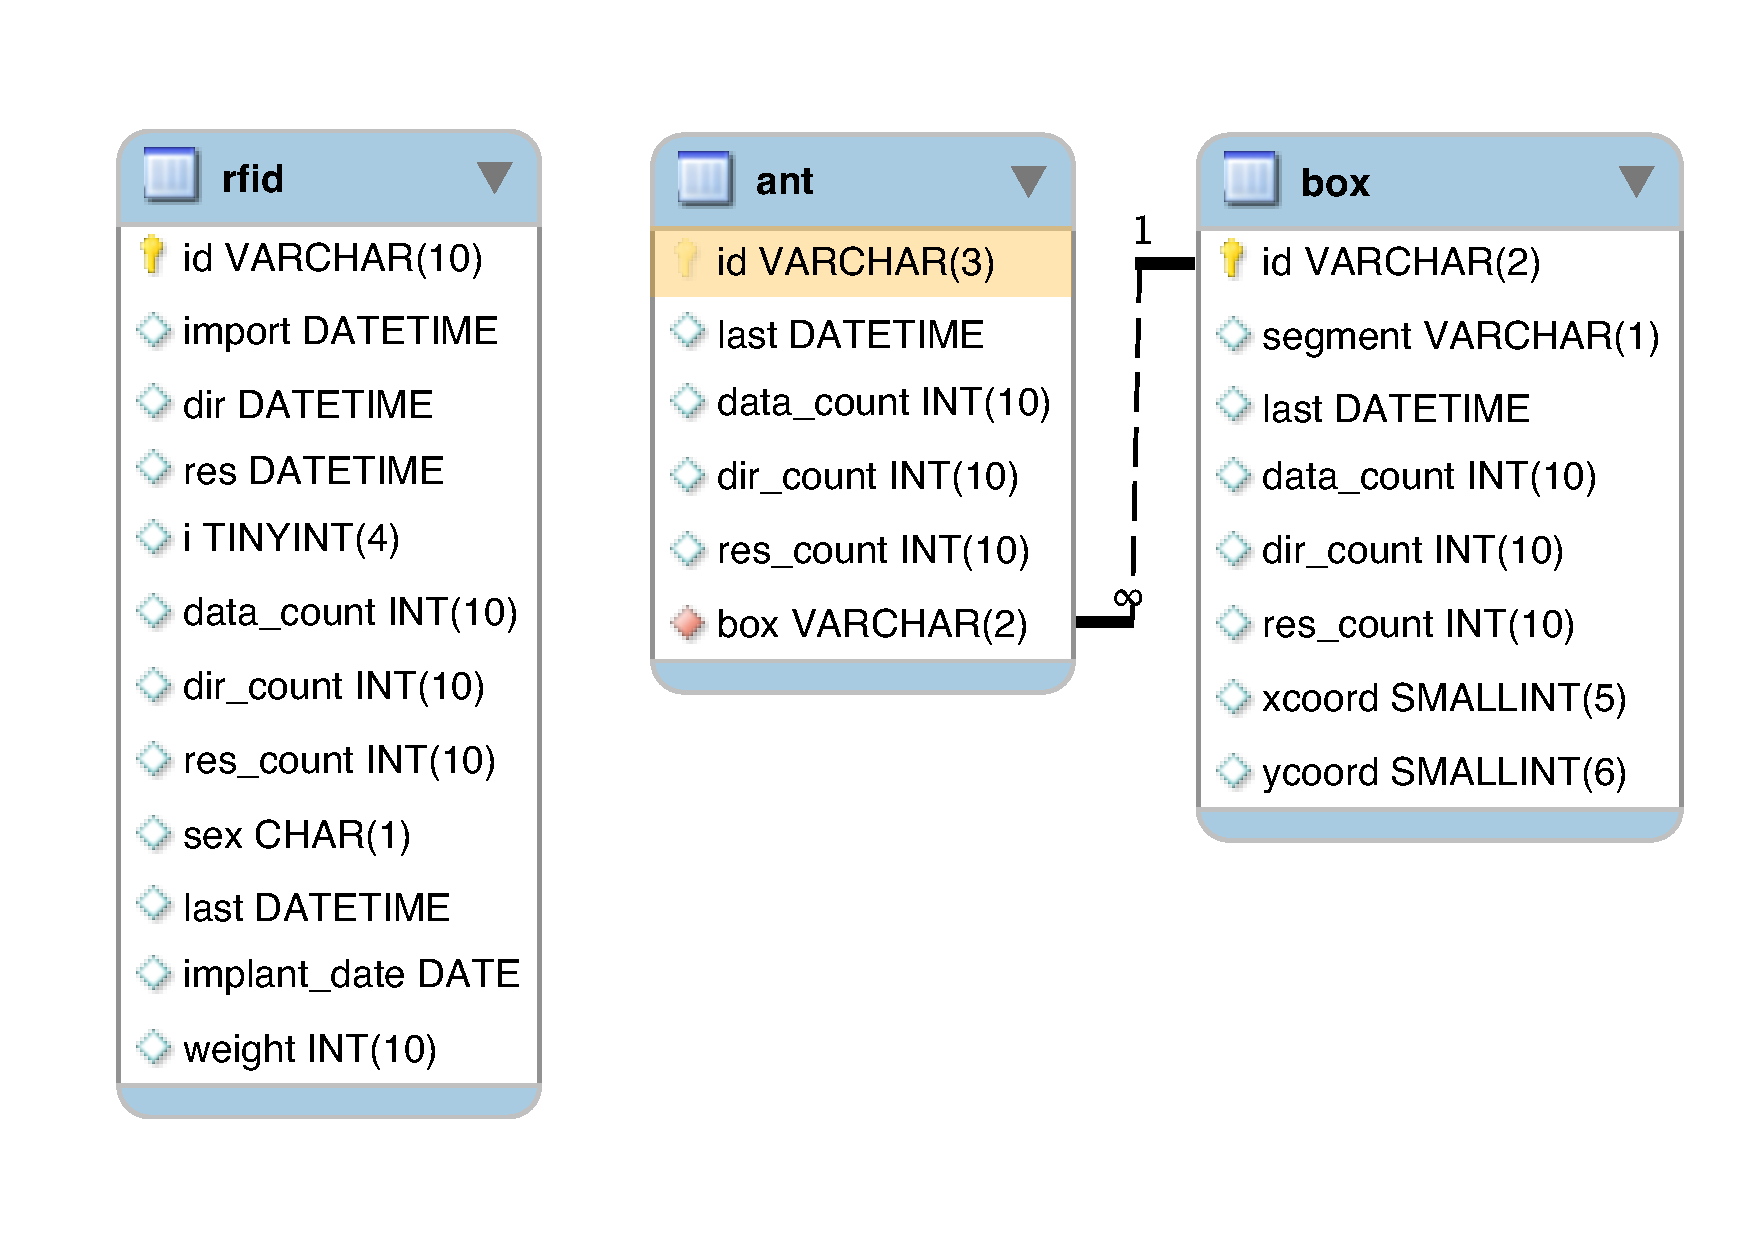
\includegraphics[width=0.75\textwidth]{assets/pdf/system_members_schema.pdf}
  \caption[Schema of database tables with system member data]{Schemata of the database tables containing the \textit{system members} data.}
  \label{fig:system_members}
\end{center}
\end{figure}

\paragraph{rfid table}
\label{para:rfid_table}

The \lstinline|rfid| table contains all the different transponder id's recorded by the system, along with the corresponding attribute data and some summarized information about each \ac{RFID}. 

Shown next is a row of the \lstinline|rfid| table followed by short explanation of the columns.
\codescript
\begin{lstlisting}[frame=none]

(first part of table row)
+------------+------+------------+-----------+-----------+
| id         | i    | data_count | dir_count | res_count |
+------------+------+------------+-----------+-----------+
| 0006955EED |    3 |          1 |         0 |         0 |
+------------+------+------------+-----------+-----------+

(second part of table row)
+------+---------------------+--------------+--------+
| sex  | last                | implant_date | weight |
+------+---------------------+--------------+--------+
| m    | 2007-08-29 23:35:41 | 2007-08-28   |   18.0 |
+------+---------------------+--------------+--------+

\end{lstlisting}

\begin{mydesc}
	\item \lstinline|id| is the unique, 10 character wide alphanumeric transpnder identification.
	\item \lstinline|i| is is a helper value used in the data import procedure. It is \lstinline|0| if new data for the transponder has been imported, \lstinline|2| if the data is searched for \textit{direction results} and \lstinline|3| if the data has been searched for results.
	\item \lstinline|data_count| contains the sum of datasets in the \lstinline|data| table.
	\item \lstinline|dir_count| contains the sum of datasets in the \lstinline|direction| table.
	\item \lstinline|res_count| contains the sum of datasets in the \lstinline|results| table.
	\item \lstinline|sex| column holds the gender of the mouse.
	\item \lstinline|last| points to the maximum value in the \lstinline|time| column of the \lstinline|data| table for this mouse. 
	\item \lstinline|implant_date| holds the date of the transponder injection.
	\item \lstinline|weight| contains a decimal number with the weight of the mouse in grams.
\end{mydesc}

\paragraph{box table}
\label{para:box_table}

The box table contains all the information about the 40 artificial nestboxes. 

Shown next is a row of the \lstinline|box| table followed by short explanation of the columns.
\codescript
\begin{lstlisting}[frame=none]

(first part of table row)
+----+---------+---------------------+------------+
| id | segment | last                | data_count |
+----+---------+---------------------+------------+
| 01 | A       | 2009-03-27 16:38:59 |     122439 | 
+----+---------+---------------------+------------+

(second part of table row)
+-----------+-----------+--------+--------+
| dir_count | res_count | xcoord | ycoord |
+-----------+-----------+--------+--------+
|     44389 |      9824 |    246 |    708 | 
+-----------+-----------+--------+--------+

\end{lstlisting}

\begin{mydesc}
	\item \lstinline|id| is the unique 2 character wide box identification.
	\item \lstinline|segment| point to the segment (A, B, C or D) the box is located in.
	\item The meaning of the \lstinline|last| \lstinline|data_count|, \lstinline|dir_count| and \lstinline|res_count| columns is already explained in the \lstinline|rfid| table.
	\item \lstinline|xcoord| and \lstinline|ycoord| contain the x (entrance side wall) and y (left wall from the entrance wall) coordinates in centimeter of the box in the barn.
\end{mydesc}

\paragraph{ant table}
\label{para:ant_table}

The ant table contains all the information about the 80 antennas. 

Shown next is a row of the \lstinline|ant| table followed by short explanation of the columns.
\codescript
\begin{lstlisting}[frame=none]
+-----+---------------------+------------+-----------+-----------+-----+
| id  | last                | data_count | dir_count | res_count | box |
+-----+---------------------+------------+-----------+-----------+-----+
| 011 | 2009-03-27 16:38:59 |      54220 |     46099 |     19648 | 01  | 
+-----+---------------------+------------+-----------+-----------+-----+

\end{lstlisting}

\begin{mydesc}
	\item \lstinline|id| is the unique 3 character wide antenna identification.
	\item The meaning of the \lstinline|last| \lstinline|data_count|, \lstinline|dir_count| and \lstinline|res_count| columns is already explained in the \lstinline|rfid| table.
	\item \lstinline|box| points to the \lstinline|id| value in the \lstinline|box| table, the antenna is attached to.
\end{mydesc}

\subsubsection{Auxiliary tables}

This group includes tables that contain percalculated data for faster data browsing with the \textit{miceminer} application and a table with the imported data files. 

\begin{figure}[htpb]
\begin{center}
  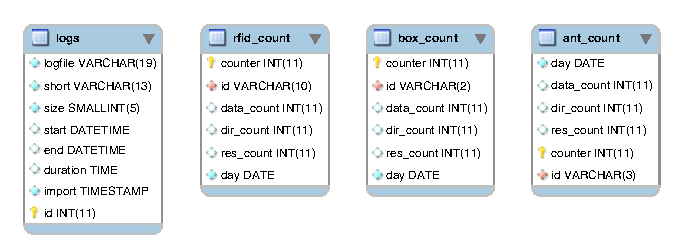
\includegraphics[width=0.75\textwidth]{assets/pdf/auxiliary_tables_schema.pdf}
  \caption[Schema of database tables with system member data]{Schemata of the database tables with the auxiliary data. The relations are not shown.}
  \label{fig:auxiliary_tables}
\end{center}
\end{figure}

\paragraph{logs table}
\label{para:logs_table} 

The \lstinline|logs| table contains information about the imported data files.

Shown next is a row of the \lstinline|logs| table followed by short explanation of the columns.

\codescript
\begin{lstlisting}[frame=none]
(first part of table row)
+-----+---------------------+---------------+------+---------------------+
| id  | logfile             | short         | size | start               |
+-----+---------------------+---------------+------+---------------------+
| 608 | 20090326_170750.txt | 09-0326170750 | 1660 | 2009-03-26 17:07:51 |
+-----+---------------------+---------------+------+---------------------+

(second part of table row)
+---------------------+----------+---------------------+
| end                 | duration | import              |
+---------------------+----------+---------------------+
| 2009-03-27 17:07:40 | 23:59:49 | 2009-04-12 01:03:01 | 
+---------------------+----------+---------------------+

\end{lstlisting}

\begin{mydesc}
	\item \lstinline|id| is the unique identifier of dataset.
	\item The original filename of the data file is stored in the \lstinline|logfile| column.
	\item \lstinline|short| values are a kind of code made up from parts of the data filename. This column was important at the beginning of the project, when we had to import data files with a different structure.
	\item \lstinline|size| contains the filesize in bytes of the data file.
	\item \lstinline|start| and \lstinline|end| indicate the first an and last point in time of an antenna reading, this data file contains.
	\item \lstinline|duration| is simply the period between the \lstinline|start| and \lstinline|end| values.
	\item \lstinline|import| refers to the time the import of the data in the file into the \lstinline|data| table was finished.
\end{mydesc}

\paragraph{rfid\_count, box\_count, ant\_count}
\label{para:counts}

These three tables contain per day data counts for transponders (\lstinline|rfid_count|), boxes (\lstinline|box_count|) and antennas (\lstinline|ant_count|), and are exclusively needed by the \textit{miceminer} application to allow faster browsing of the data.

Shown next is a row of the \lstinline|rfid_count|, \lstinline|box_count|, \lstinline|ant_count| tables followed by short explanation of the columns.

\codescript
\begin{lstlisting}[frame=none]
(row of table rfid_count)
+---------+------------+------------+------------+-----------+-----------+
| counter | id         | day        | data_count | dir_count | res_count |
+---------+------------+------------+------------+-----------+-----------+
|     999 | 0006B9C5E8 | 2008-07-14 |         10 |         4 |         2 | 
+---------+------------+------------+------------+-----------+-----------+


(row of table box_count)
+---------+----+------------+------------+-----------+-----------+
| counter | id | day        | data_count | dir_count | res_count |
+---------+----+------------+------------+-----------+-----------+
|     999 | 10 | 2008-07-31 |        259 |       114 |        39 | 
+---------+----+------------+------------+-----------+-----------+


(row of table ant_count)
+---------+-----+------------+------------+-----------+-----------+
| counter | id  | day        | data_count | dir_count | res_count |
+---------+-----+------------+------------+-----------+-----------+
|     999 | 121 | 2008-07-19 |        196 |       174 |        47 | 
+---------+-----+------------+------------+-----------+-----------+


\end{lstlisting}

\begin{mydesc}
	\item \lstinline|counter| is the unique identifier of dataset.
	\item \lstinline|id| contains the identification of the transponder, the box or the antenna.
	\item \lstinline|day| points to the day the table row holds the data counts for.
	\item \lstinline|data_count|, \lstinline|dir_count| and \lstinline|res_count| contain the per day countes for the datasets, the \textit{direction results} and the \textit{stay results}.
\end{mydesc}

\subsection{Data access}
\label{subsec:dataccess}

Most of the mainly used relational databases offer \ac{SQL} (SQL) to manage and retrive the data. However, SQL is not easy to learn and use, lacks built-in export functionality of the data to file formats such as $Microsoft Excel^{\copyright}$, and does not offer any possibility to visualize the data. Therefore, a feature rich but still handy and intuitive, \ac{GUI} (GUI) is available, making it easy for the user to explore, visualize and export data (see section \ref{subsec:dataexp} on page \pageref{subsec:dataexp}).